% !TEX root = ../main.tex
%

\chapter{大域最適化}

勾配を用いた最適化アルゴリズムでは、
局所的に目的関数が周りより小さい点(局所最適解)を見つけられるが、
目的関数が最も小さくなる点(大域最適解)を見つけられるとは限らない。
そこで、大域最適解を求める大域最適化のアルゴリズムが考えられている。
本章では大域最適化のアルゴリズムについてまとめる。

\section{Dividing Rectangles (DIRECT) 法}

Dividing Rectangles (DIRECT) 法 \cite{Jones1993} では、
黄金比探索(第 \ref{sec:optimization_golden-section-search} 節)と同様に
領域を分割していきながら最適解を求める。
ただし、黄金比探索と異なり大域最適解を求めるため、
目的関数の値が小さくない点も一定の条件でさらに分割していく。

DIRECT 法では、
探索領域を $n$ 次元単位超立方体 $[0, 1]^n$ とし、
その上で定義される目的関数 $f : [0, 1]^n \to \setR$ を考える。
目的関数は Lipschitz 連続であるとする。
つまり、ある定数 $K$ が存在し、
任意の点 $\bm{x}, \bm{y} \in [0, 1]^n$ について
\begin{equation}
    |f(\bm{x}) - f(\bm{y})| \le K \|\bm{x} - \bm{y}\|_2
\end{equation}
が成り立つとする。
アルゴリズムの進行とともに探索領域は超短形
\footnote{ここで扱う超短形 (hyper-rectangle) は%
$[a_1, b_1] \times [a_2, b_2] \times \ldots \times [a_n, b_n]$%
のように区間の積で示される領域である。}
に分割されていくが、次に分割する超短形を決定するために、
次のような「最適な可能性のある超短形」を定義する。

\begin{definition}[{\cite[Definition 4.1.]{Jones1993}}]
    \label{def:optimization_direct_potentially-optimal}
    反復により探索領域が $m$ 個の超短形に分割されているものとし、
    $i$ 番目の超短形の中心点を $\bm{c}_i$ とする。
    $j$ 番目の超短形が次の条件を満たすような定数 $\tilde{K}$ が存在する場合、
    最適な可能性のある超短形と呼ぶ。
    \begin{align}
        f(\bm{c}_j) - \tilde{K} d_j &\le f(\bm{c}_i) - \tilde{K} d_i & \text{for all $i = 1, \ldots, m$}
        \label{eq:optimization_direct_potentially-optimal_smaller-than-others}
        \\
        f(\bm{c}_j) - \tilde{K} d_j &\le f_{\text{min}} - \epsilon |f_{\text{min}}|
        \label{eq:optimization_direct_potentially-optimal_smaller-than-now}
    \end{align}
    ここで、$f_{\text{min}} = \min{\{f_i \mid i = 1, \ldots, m\}}$ であり、
    $d_i$ は $i$ 番目の超短形の中心から端点までの距離であり、
    $\epsilon$ は正の実数の定数である。
\end{definition}

$f(\bm{c}_j) - \tilde{K} d_j$ は
Lipschitz 定数が $\tilde{K}$ である場合に $j$ 番目の超短形の中で取り得る最小値を示す。
そのため、
式 \eqref{eq:optimization_direct_potentially-optimal_smaller-than-others} は、
Lipschitz 定数が $\tilde{K}$ である場合に
最も小さい値を取り得る超短形が $j$ 番目の超短形であることを示す。
式 \eqref{eq:optimization_direct_potentially-optimal_smaller-than-now} は、
Lipschitz 定数が $\tilde{K}$ である場合に、
$j$ 番目の超短形で現状の大域最適解を
少なくとも $\epsilon |f_{\text{min}}|$ だけ更新する可能性があることを示す。

\begin{figure}[tp]
    \centering
    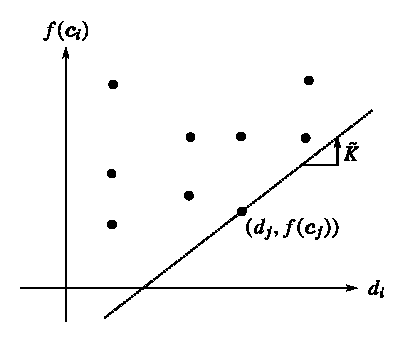
\includegraphics[width=0.7\linewidth]{optimization/DIRECT-potentially-optimal.pdf}
    \caption{式 \eqref{eq:optimization_direct_potentially-optimal_smaller-than-others_rewritten} のイメージ}
    \label{fig:optimization_direct_potentially-optimal_smaller-than-others-image}
\end{figure}

超短形を分割する場合、
各軸の区間の長さを比べて長い方向から分割するようにし、
最も長い軸が複数ある場合は次元の小さい方から順に分割することで、
分割数の同じ超短形は同じ形状になるようにする。
これにより、分割数の同じ超短形は
定義 \ref{def:optimization_direct_potentially-optimal} における $d_i$ が同じになり、
分割数の同じ超短形同士では
式 \eqref{eq:optimization_direct_potentially-optimal_smaller-than-others}
が単に目的関数の大小により評価できるようになる。
また、式 \eqref{eq:optimization_direct_potentially-optimal_smaller-than-others} は
\begin{equation}
    f(\bm{c}_i) \ge f(\bm{c}_j) + \tilde{K} (d_i - d_j)
    \label{eq:optimization_direct_potentially-optimal_smaller-than-others_rewritten}
\end{equation}
のように書くこともでき、
図 \ref{fig:optimization_direct_potentially-optimal_smaller-than-others-image}
のように他の点が全て上に来るような直線を引けることを示す。
このような点を探すアルゴリズムは凸包探索として知られる。

\begin{algorithm}[tp]
    \caption{DIRECT 法}
    \label{alg:optimization_direct}
    \begin{algorithmic}
        \Procedure{DIRECT}{$f, ,\epsilon$}
            \State 単位超立方体 $[0, 1]^n$ を最初の超短形とする
            \Loop
                \State 凸包探索を用いて
                    式 \eqref{eq:optimization_direct_potentially-optimal_smaller-than-others_rewritten}
                    を満たす超短形を探索する
                \State 式 \eqref{eq:optimization_direct_potentially-optimal_smaller-than-now}
                    を満たさない超短形は除外する
                \State 残った超短形を最も長い軸に沿って 3 つに分割する
                \If{停止条件を満たす場合}
                    \State \Return
                \EndIf
            \EndLoop
        \EndProcedure
    \end{algorithmic}
\end{algorithm}

ここまでの議論により、DIRECT 法は
Algorithm \ref{alg:optimization_direct} のようになる。
停止条件としては、反復回数が用いられる。

DIRECT 法の派生としては以下のようなものが挙げられる。

\begin{itemize}
    \item 各局所最適解への収束に重点をおいた DIRECT-l \cite{Gablonsky2001}
\end{itemize}
